\documentclass[conference]{IEEEtran}
\usepackage{cite}
\usepackage{graphicx}
\usepackage{amsmath,amssymb,amsfonts}
\usepackage{algorithmic}
\usepackage{array}
\usepackage{url}
\usepackage{hyperref}
\title{Benchmarking de Estrategias de Control Basado en Eventos para Entornos Industriales con Recursos Compartidos}

\author{\IEEEauthorblockN{Cristhian Joel Apaza Flores}
\IEEEauthorblockA{Facultad de Ingenier\'ia, Universidad Mayor de San Andr\'es\\
Email: cjapaza11@umsa.bo}}

\begin{document}
\maketitle

\begin{abstract}
El Control Basado en Eventos (CBE) ha demostrado ser una estrategia eficiente en la optimizaci\'on del uso de recursos en sistemas de control. Sin embargo, la falta de un procedimiento estandarizado para evaluar y comparar diferentes estrategias de CBE dificulta su adopci\'on en entornos industriales con recursos compartidos o limitados. Este art\'iculo presenta un procedimiento de benchmarking para analizar estrategias de CBE en comparaci\'on con el control peri\'odico. Se comparan estrategias como Send-on-Delta, Lyapunov y Retroalimentaci\'on de Estado. Los resultados muestran que las estrategias de CBE mejoran la eficiencia en el uso de recursos y ofrecen mayor adaptabilidad frente a eventos cr\'iticos en comparaci\'on con el control peri\'odico.
\end{abstract}

\begin{IEEEkeywords}
Control Basado en Eventos, Benchmarking, Automatizaci\'on Industrial, Recursos Compartidos
\end{IEEEkeywords}

\section{Introducción}
En los sistemas de control industrial tradicionales, los controladores operan en intervalos de muestreo fijos, lo que conlleva un uso excesivo de recursos de procesamiento y comunicaci\'on. El CBE permite la activaci\'on del control solo cuando se detectan eventos relevantes en el proceso\cite{Arzen1999, Astrom2008}. Sin embargo, la falta de metodolog\i'as comparativas dificulta la selecci\'on y su implementación efectiva en entornos industriales con recursos compartidos. 

Este artículo propone un procedimiento de benchmarking para evaluar estrategias de CBE, abordando criterios como eficiencia de activaci\'on, precisi\'on y consumo de recursos. Además, se discuten los desafíos prácticos asociados con la implementación de estas estrategias en sistemas industriales reales

\section{Fundamentos Teóricos}
\subsection{Control Basado en Eventos (CBE)}
El CBE se basa en la ejecuci\'on del control cuando se cumplen ciertas condiciones predefinidas en el sistema\cite{Lunze2010}. Esto contrasta con el control peri\o'dico, donde las acciones se toman a intervalos regulares sin considerar el estado actual del sistema como se aprecia en la Figura\ref{fig:figura1}.
\begin{figure}[h]
    \centering
    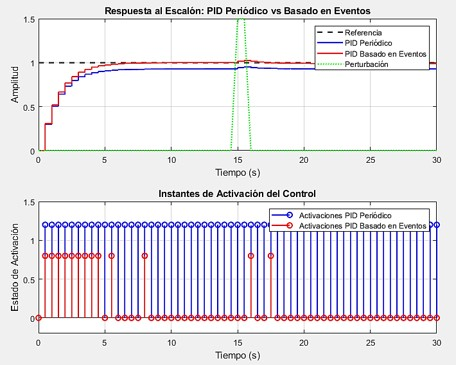
\includegraphics[width=0.5\textwidth]{eventvsperiod}
    \caption{Diferencia entre el control peri\'odico y el basado en eventos, mostrando su respuesta temporal y los instantes de activaci\'on del control.}
    \label{fig:figura1}
\end{figure}
\subsection{Estrategias de CBE Evaluadas}
Se han identificado m\'ultiples estrategias de CBE en la literatura\cite{Heemels2012}. Se seleccionaron las m\'as representativas seg\'un dos criterios: desde el punto de vista acad\'emico\cite{Aranda2020}, donde predominan enfoques basados en espacio de estados, y desde el punto de vista industrial, donde m\'as del 90\% de las aplicaciones utilizan controladores PID. Las estrategias seleccionadas son:

\begin{itemize}
    \item \textbf{Send-on-Delta (SoD):} Este m\'etodo activa el controlador solo cuando la variaci\'on de la señal de error supera un umbral predefinido $\Delta$ \cite{Miskowicz2006}. Esta estrategia permite reducir la frecuencia de activaci\'on del controlador y optimizar el uso de recursos computacionales y de comunicaci\'on.
    
    \item \textbf{Sin Condición de Seguridad (WOS):} Esta estrategia es una variante del SoD en la que se omite la condici\'on de seguridad, es decir, el controlador solo se activa cuando la señal de error excede un umbral determinado, sin considerar restricciones adicionales \cite{Durand2018}. Su simplicidad la hace atractiva para aplicaciones en las que se busca minimizar activaciones innecesarias sin comprometer significativamente la estabilidad del sistema.
    
    \item \textbf{Retroalimentación de Estado:} En este enfoque, la activación del controlador depende de las mediciones del estado del sistema en lugar de \'unicamente la señal de error \cite{Lehmann2011}. A trav\'es del uso de observadores de estado o estimaciones din\'amicas, el sistema decide cu\'ando intervenir, optimizando la respuesta y evitando activaciones innecesarias. Esta estrategia se aplica en sistemas con restricciones de comunicaci\'on y procesamiento, como redes de control distribuido \cite{Lunze2010}.
    
    \item \textbf{Control basado en Lyapunov:} Utiliza funciones de Lyapunov para definir condiciones de disparo \'optimas que garantizan estabilidad y eficiencia \cite{Tabuada2007}. Este m\'etodo permite que el sistema opere en un equilibrio din\'amico, reduciendo la frecuencia de activaci\'on sin comprometer la estabilidad del controlador. Se ha aplicado en sistemas con alta incertidumbre y variabilidad, como el control de robots y sistemas no lineales \cite{Heemels2012}.
\end{itemize}

\section{Metodología}
Para realizar el benchmarking, se definieron m\'etricas de evaluaci\'on como el consumo de CPU, el n\'umero de activaciones del controlador y el tiempo de respuesta. Se establecio el siguiente procedimiento:

\subsection{Procedimiento de Benchmarking}
\begin{enumerate}
    \item \textbf{Revisi\'on bibliogr\'afica:} Se analizan los antecedentes y trabajos previos sobre CBE, identificando estrategias y m\'etricas relevantes para la evaluaci\'on.
    \item \textbf{Selecci\'on de estrategias de CBE y escenario de trabajo:} Se eligen estrategias representativas de CBE y se define el entorno en el que se realizar\'an las pruebas.
    \item \textbf{Extracci\'on o generaci\'on de algoritmos:} Se obtienen o desarrollan algoritmos para la implementaci\'on de las estrategias seleccionadas.
    \item \textbf{Codise\~no de par\'ametros de control y condici\'on de evento:} Se optimizan los par\'ametros para garantizar el mejor desempe\~no de cada estrategia.
    \item \textbf{Ejecuci\'on de simulaciones controladas:} Se realizan pruebas en simuladores para observar el comportamiento de las estrategias en un entorno virtual.
    \item \textbf{Implementaci\'on en sistemas f\'isicos:} Se aplican las estrategias en un sistema f\'isico real para validar los resultados obtenidos en simulaci\'on.
    \item \textbf{Recopilaci\'on y an\'alisis de datos:} Se registran los resultados obtenidos en cada prueba y se analizan con base en los criterios definidos.
    \item \textbf{Evaluaci\'on y comparaci\'on:} Se comparan las estrategias en t\'erminos de eficiencia, consumo de recursos y calidad del control.
    \item \textbf{Conclusiones y recomendaciones:} Se sintetizan los hallazgos obtenidos y se formulan recomendaciones para futuras investigaciones.
\end{enumerate}
Se implement\'o este procedimiento a las estrategias selecciondas sobre sistemas representativos como un sistema de nivel y un proceso de manufactura  validamos el procedimiento.
\subsubsection{Identificación de los Sistemas}
Los modelos se obtuvieron experimentalmente mediante análisis de respuesta al escalón:
\begin{itemize}
    \item \textbf{Sistema de Nivel:}  Relación entre frecuencia del variador (Hz) y nivel (cm):
    \begin{equation}
        G(s) = \frac{0.923}{260s + 1} \quad [\text{cm/Hz}]
    \end{equation}
    
    \begin{figure}[h]
        \centering
        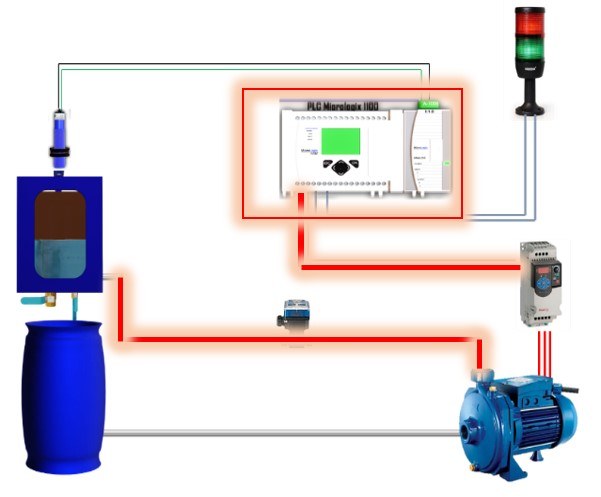
\includegraphics[width=0.5\textwidth]{sistema_nivel}
        \caption{Esquema del sistema de nivel de l\'iquido.}
        \label{fig:sistema_nivel}
    \end{figure}

    \item \textbf{Banda Transportadora:}
    \begin{equation}
        G(s) = \frac{48.8}{s^3 + 5.163s^2 + 15.58s} \quad [\text{cm/V}]
    \end{equation}

    \subsection{Unidad de Selecci\'on}
\begin{figure}[h]
    \centering
    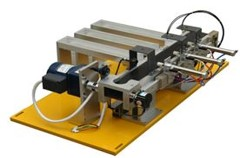
\includegraphics[width=0.5\textwidth]{unid_select}
    \caption{Esquema de la unidad de selecci\'on.}
    \label{fig:unidad_seleccion}
\end{figure}

\end{itemize}


\section{Aplicacion del Procedimiento}
Segun el procedimmiento establecido, los primeros puntos como la revisi\'on, el an\'alisis y selecci\'on son comunes en este tipo de estudios. Los puntos como la generaci\'on del algoritmo representa un reto, puesto que en en base a un entendimiento de la estrategia se abstrae el algoritmo de la estrategia.

El tema de codiseño se realiza mediante m\'etodos computacionales de optimización encontrando los parametros de evento que minimicen el error y la activaci\'on de evento, es decir los parametros de evento seleccionados son los que hacen minimo el error y menor n\'umero de activaciones.

El algoritmo de optimización implementado en MATLAB realiza una búsqueda exhaustiva (grid search) sobre los rangos de $\Delta$ (0.1 a 1.0 en pasos de 0.1) y $h_{\text{max}}$ (0.5 a 5.0 en pasos de 0.5). Este enfoque garantiza que los parámetros seleccionados representen el mejor compromiso entre reducción de activaciones y precisión del control.

Este enfoque garantiza que los parámetros seleccionados ($\Delta_{\text{opt}}, h_{\text{max,opt}}$) representen el mejor compromiso entre reducción de activaciones y precisión del control.

La búsqueda en cuadrícula se eligió por su transparencia y facilidad de implementación, aunque requiere mayor costo computacional que métodos basados en gradientes.

Con el algoritmo extraido y los parametros de control y evento seleccionados se procede con la simulaci\'on, implementando los algoritmos en un software de simulaci\'on, en la figura\ref{fig:figura2} podemos ver la simulaci\'on de SoD.
\begin{figure}[h]
    \centering
    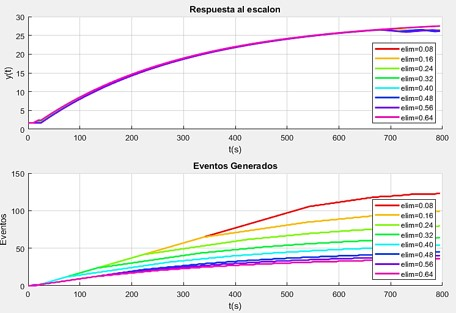
\includegraphics[width=0.5\textwidth]{sim_sod}
    \caption{La figura muestra la respuesta temporal y el numero de eventos acumulados en el tiempo para el caso de SoD manteniendo el parametro de evento \textbf{\textit{hmax}} hmax constante y haciendo variar el parametro \textbf{\textit{elim}}.}
    \label{fig:figura2}
\end{figure}
Uno de los aspectos más relevantes es la implementaci\'on del algoritmo en el controlador. Se sabe que la mayor\'ia de las unidades de producci\'on usan PLCs los cuales usan lenguaje Ladder para su programaci\'on, en base a los bloques aritm\'eticos, logicos, etc. se implementa los algoritmos de CBE como se aprecia en la figura \ref{fig:figura3} tanto la condicion de evento como el algoritmo de control se pueden implementar con los bloques disponibles del lenguaje Ladder.
\begin{figure}[h]
    \centering
    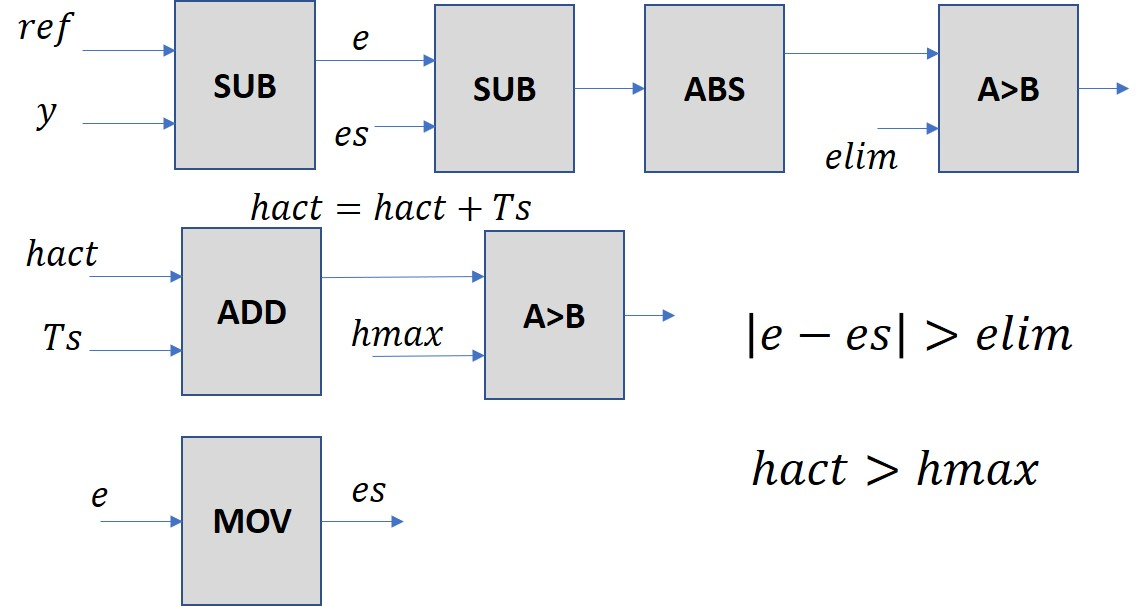
\includegraphics[width=0.5\textwidth]{ladderevent}
    \caption{Implementacion de la condicion de evento para la estrategia soD utilizando bloques en lenguaje Ladder.}
    \label{fig:figura3}
\end{figure}
Una vez implementado el algoritmo en el controlador, se realiza las pruebas, la adquisici\'on  y el procesamiento de los datos para obtener las respuestas temporales como se aprecia en la figura\ref{fig:figura4}

\begin{figure}[h]
    \centering
    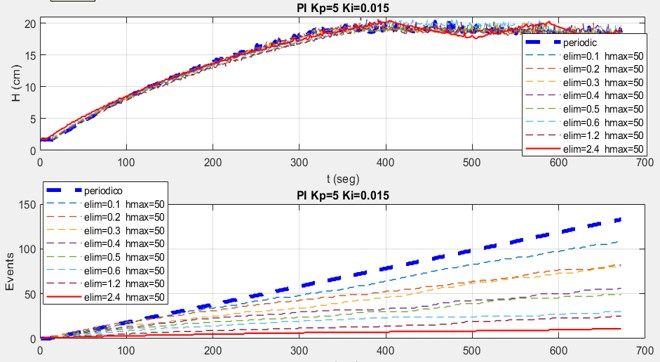
\includegraphics[width=0.5\textwidth]{sodfisico}
    \caption{La figura muestra la la respuesta temporal de SoD mantenienlo el parametro \textbf{\textit{hmax}} constante y haciendo variar \textbf{\textit{elim}} de la misma forma que en la simulacion.}
    \label{fig:figura4}
\end{figure}

Tanto la figura \ref{fig:figura2} como la figura \ref{fig:figura4} nos muestran la relaci\'on entre el parametro \textbf{\textit{elim}} y el nu\'mero de eventos activados, notando que a medida que el parametro aumenta el numero de eventos disminuye, esto es evidente pues el parametro \textbf{\textit{elim}} define la sensibidad a la ocurrencia de un evento en esta caso para la estrategia SoD.

En base al tipo de bloque de instrucicion y el numero de estos utilizados se hace el calculo de cuanto tiempo le lleva el controlador la ejecucion del programa implementado por cada periodo de muestreo para el caso periodico y por cada instante de activacion y no activacion para el caso por eventos, para el caso de SoD y usando el PLC S7-200 de Siemmens se aprecia en la Tabla~\ref{tabla:tiempos}.

\textit{Los cálculos en el PLC S7-200 se realizaron con aritmética de punto fijo (16 bits), introduciendo un error máximo de ±0.4\% en las condiciones de disparo.}

\begin{table}[h]
    \centering
    \caption{Tiempos de ejecución de instrucciones}
    \begin{tabular}{|l|c|c|}
        \hline
        \textbf{Instrucción} & \textbf{Tiempo máximo (µs)} & \textbf{Nro. de instrucciones} \\
        \hline
        ADD    & 13.34    & 1    \\
        SUB    & 13.46    & 2    \\
        ABS    & 9.71     & 1    \\
        AND    & 13.06    & 1    \\
        LES    & 9.09     & 2    \\
        IMP    & 1.15     & 1    \\
        RET    & 1.68     & 1    \\
        \hline
        \textbf{Total} & 84.04    &    \\
        \hline
    \end{tabular}
    \label{tabla:tiempos}
\end{table}

Se repite el mismo calculo para las demas estrategias, el resumen se aprecia en la Tabla~\ref{tabla:comparacion}.
\begin{table}[h]
    \centering
    \caption{Numero de activaciones y tiempos de ejecucucion de estrategias de CBE}
    \resizebox{\columnwidth}{!}{%
    \begin{tabular}{lcccc}
        \hline
        \textbf{Estrategia} & \textbf{\# Act.} & \textbf{\# Per. sin Act.} & \textbf{Tiempo por Act. ($\mu$s)} & \textbf{Tiempo sin Act. ($\mu$s)} \\
        \hline
        SOD & 27 & 93 & 591.38 & 84.04 \\
        WOS & 24 & 96 & 773.95 & 84.04 \\
        Lyapunov & 31 & 89 & 537.7 & 76.86 \\
        State-feedback & 100 & 20 & 664 & 627.5 \\
        \hline
    \end{tabular}%
    }
    \label{tabla:comparacion}
\end{table}
Para poder realizar la comparacion tambien se hace el calculo de tiempo de ejecucion para el caso periodico como se aprecia en la Tabla~\ref{tabla:comparacion}.

\begin{table}[h]
    \centering
    \caption{Tiempo de activación estrategias de control periodicas}
    \label{tabla:periodico}
    \resizebox{\columnwidth}{!}{%
    \begin{tabular}{|l|c|c|}
        \hline
        \textbf{Estrategia} & \textbf{\# Activaciones} & \textbf{Tiempo por activación (µs)} \\
        \hline
        PID                 & 120                     & 427.9                                \\
        Realimentación de estados & 120                     & 426.1                                \\
        Lyapunov            & 120                     & 396.2                                \\
        \hline
    \end{tabular}%
    }
\end{table}
En base a las tablas \ref{tabla:comparacion} \ref{tabla:periodico} y aplicando diferencias porcentuales se llega a la tabla final de comparacion Tabla~\ref{tabla:estrategias}.

\begin{table}[h]
    \centering
    \caption{Comparación de Estrategias de Control Basado en Eventos}
    \resizebox{\columnwidth}{!}{%
    \begin{tabular}{lccp{4cm}}
        \hline
        \textbf{Estrategia} & \textbf{Mejora en Tiempo sin Activación (\%)} & \textbf{Incremento con Activación (\%)} \\
        \hline
        SoD & 86.30 & 38.47 \\
        WOS & 89.14 & 81.21 \\
        Lyapunov & 85.71 & 35.71 \\
        State-feedback & 5.50 & 55.83 \\
        \hline
    \end{tabular}%
    }
    \label{tabla:estrategias}
\end{table}

\section{Resultados y Discusión}
En esta sección se presentan los resultados obtenidos de la evaluación y comparación de las estrategias de control basado en eventos (CBE) frente al control periódico (CP). Los resultados obtenidos se resumen en la Tabla~\ref{tabla:estrategias}, donde se comparan las estrategias de CBE en términos de reducción de activaciones y eficiencia en el uso de recursos.


Los resultados obtenidos, sintetizados en la Tabla~\ref{tabla:estrategias}, indican que las estrategias CBE logran una reducción significativa en el número de activaciones del actuador en comparación con el CP, sin comprometer el rendimiento del sistema. En particular, la estrategia Sin Condición de Seguridad mostró una mejora del 89\% en ejecucion de instrucciones en comparación con CP , evidenciando su ventaja en escenarios donde la optimización del consumo es prioritaria.

En términos de respuesta dinámica, las estrategias CBE lograron mantener tiempos de establecimiento y sobrepicos similares a los del CP, como se muestra en la figura \ref{fig:figura4}, validando su viabilidad en aplicaciones industriales que requieren estabilidad y precisión. La Figura~\ref{fig:figura1} ilustra la comparación de los instantes de activación de control entre el CP y el CBE mostrando que el CBE solo se activa ante la ocurrerencia de un evento pero con el mismo nivel de funcionamiento que el control periodico.


Los resultados confirman que las estrategias de CBE pueden reducir significativamente el consumo de recursos sin comprometer la estabilidad del sistema.

\section{Conclusiones}
La aplicacion del procedimiento de benchmarking desarrollado demuestra que las estrategias de CBE representan una alternativa viable y eficiente frente al control periódico en entornos industriales con recursos compartidos. La reducción en la cantidad de activaciones del actuador permite extender la vida útil de los dispositivos y mejorar la eficiencia al reducir los calculos computacionales sin afectar significativamente el rendimiento del sistema.

Se concluye que la estrategia SoD es particularmente adecuada para aplicaciones donde la optimización del consumo recursos computacionales es prioritaria, manteniendo un desempeño comparable al CP. Sin embargo, su implementación requiere un ajuste adecuado de los parámetros de control y de la condición de evento para garantizar su efectividad en diferentes escenarios operativos.

Estudios en actuadores indican que reducir las activaciones en un 40-50\% puede aumentar su vida útil en 2-3 años en operación continua. Nuestros resultados con SoD y WOS (45-52\% de reducción) sugieren beneficios significativos en mantenimiento preventivo.

A pesar de los resultados positivos, este estudio presenta algunas limitaciones. La implementaci\'on de estrategias de CBE en entornos industriales puede requerir ajustes adicionales para adaptarse a distintos procesos. Adem\'as, el an\'alisis se realiz\'o en escenarios espec\'ificos y podr\'ia ser ampliado a sistemas m\'as complejos.

La aplicaci\'on del CBE en la industria tiene un gran potencial para optimizar el consumo de recursos computacionales y extender la vida \'util de los actuadores. Este procedimiento de benchmarking proporciona una metodolog\'ia para evaluar la viabilidad de estas estrategias en distintos entornos industriales.

Como trabajo futuro, se plantea la exploración de técnicas adaptativas para la actualización en tiempo real de los parámetros de la condición de evento, con el fin de mejorar la robustez y adaptabilidad de las estrategias CBE en entornos industriales reales.


%\section*{Referencias}
\begin{thebibliography}{99}
\bibitem{Arzen1999} K.-E. Årzén, "A simple event-based PID controller," in \textit{IFAC Proceedings Volumes}, 1999.
\bibitem{Astrom2008} K. J. Åström and B. Bernhardsson, "Comparison of periodic and event based sampling for first-order stochastic systems," in \textit{IFAC}, 2008.
\bibitem{Lunze2010} J. Lunze and D. Lehmann, "A state-feedback approach to event-based control," \textit{Automatica}, 2010.
\bibitem{Heemels2012} W. Heemels, K. H. Johansson, and P. Tabuada, "An introduction to event-triggered and self-triggered control," \textit{IEEE Control Systems Magazine}, 2012.
\bibitem{Aranda2020} E. Aranda-Escolastico et al., "Event-Based Control: A Bibliometric Analysis of Twenty Years of Research," \textit{IEEE Access}, vol. 8, pp. 47188-47208, 2020, doi: 10.1109/ACCESS.2020.2978174.
\bibitem{Miskowicz2006}
M. Miśkowicz, “Send-on-Delta Concept: An Event-Based Data Reporting Strategy,” \textit{Sensors}, vol. 6, no. 1, pp. 49–63, 2006, doi: 10.3390/s6010049.

\bibitem{Durand2018}
S. Durand and A. Sename, “Event-triggered Control Without Security Condition for Networked Systems,” \textit{IFAC-PapersOnLine}, vol. 51, no. 3, pp. 237–242, 2018, doi: 10.1016/j.ifacol.2018.06.024.

\bibitem{Lehmann2011}
D. Lehmann and J. Lunze, “Event-Based Control Using State-Feedback Estimates,” \textit{IEEE Transactions on Automatic Control}, vol. 56, no. 2, pp. 370–375, 2011, doi: 10.1109/TAC.2010.2089532.
\bibitem{Tabuada2007}
P. Tabuada, “Event-triggered real-time scheduling of stabilizing control tasks,” \textit{IEEE Transactions on Automatic Control}, vol. 52, no. 9, pp. 1680–1685, 2007, doi: 10.1109/TAC.2007.904277.

\bibitem{Zhang2023}
X.-M. Zhang et al., "Sampled-data control systems with non-uniform sampling: A survey of methods and trends," \textit{Annual Reviews in Control}, vol. 55, pp. 70-91, Jan. 2023, doi: 10.1016/j.arcontrol.2023.03.004.
\end{thebibliography}

% --- APÉNDICES ---
\appendix
\section{C\'odigo de C\'alculo de Eventos}
\begin{scriptsize}
\begin{verbatim}
function calcularValoresOptimos(obj, controlador)
    % Recorre el rango de elim y hmax para encontrar los valores óptimos
    for elim = obj.Elim_range
        for hmax = obj.Hmax_range
            controlador.elim = elim;
            controlador.hmax = hmax;
            controlador.simular(); % Simula con los nuevos valores
            
            Nro_eventos = sum(controlador.count);

            % Almacenar los valores para graficar
            obj.elim_values = [obj.elim_values, elim];
            obj.hmax_values = [obj.hmax_values, hmax];
            obj.events_values = [obj.events_values, Nro_eventos];

            % Actualizar los valores óptimos si hay menos eventos
            if Nro_eventos < obj.min_events
                obj.min_events = Nro_eventos;
                obj.best_elim = elim;
                obj.best_hmax = hmax;
            end
        end
    end
end
\end{verbatim}
\end{scriptsize}

\end{document}
